
\section{Numerical Experiment}\label{sec:experiment}
\subsection{Experimental Settings}\label{subsec:exp-settings}
	In this section, we numerically evaluate the proposed DRCS through experiments.
	%
	For this experiment, $\bm \beta_{\bm 1_n, \bm 1_n}^{*}, \bm \alpha_{\bm 1_n, \bm 1_n}^{*}$ is learned by solving \eqref{eq:primal} and \ref{eq:dual}.
	%
	We perform cross-validation with a training-to-test data ratio of 4:1 in the experiments.
	%
	Next, we define the training weight range as ${\cal W} := \left\{ \bm w \mid \left\|\bm w - \bm 1_n\right\|_2\leq S \right\}$ and set $S$ as follows.
	%
	The datasets are primarily designed for binary classification, and for multi-class datasets, two classes are extracted and used.
	%
	We set $S$ with a parameter $a$ as $S = \sqrt{n^+}|a - 1|$, where $n^+$ is the number of positive instances in the training dataset. We defined as above since it is equivalent to the case when the class balance is changed; if the weights of all positive instances (${i \mid y_i = +1}$) change from 1 to $a$ while the weights for negative instances (${i \mid y_i = -1}$) remain at 1, $S$ is calculated as above. $a = 1$ means that no distribution change occurs.
	%We assume that the weights for positive instances (${i \mid y_i = +1}$) change from 1 to $a$, while the weights for negative instances (${i \mid y_i = -1}$) remain at 1.
	%
	%The magnitude of this weight change is then defined as $S$. Specifically, we set $S = \sqrt{n^+}|a - 1|$, where $n^+$ is the number of positive instances in the training dataset.
	%
	%With this setup, $\bm w$ is allowed to vary within the range of weight changes up to $S$, permitting all weight fluctuations with a magnitude of $S$.
	%
	Similarly, we define the validation weight range as ${\cal W}' := \left\{ \bm w' \mid \left\|\bm w' - \bm 1_n\right\|_2\leq Q \right\}$ and set $Q$ in the same way as above.
	%
	In the learning setup of this paper, we adopt the empirical risk minimization approach as shown in \eqref{eq:primal}, and thus the regularization parameter $\lambda$ is determined based on the number of instances.
	%
	Specifically, we first present results obtained by retraining with $\lambda$ that is determined by cross-validation. Results for other values of $\lambda$ will be discussed later in Section \ref{subsec:discussion-lambda}.
	%
	Details of implementations are presented in Appendix~\ref{app:implementation}, and details of data setups and hyperparameters are presented in Appendix~\ref{app:experimental-setup}.


	\subsection{Coreset Selection for Tabular Data}
	\label{subsec:result-table}

	In this section, we present the experimental results for tabular datasets.
	%
	The experiments in this section were conducted using a logistic regression model (logistic loss + L2 regularization), with Radial Basis Function (RBF) kernels
	\footnote{Hyperparameters of RBF kernel are determined with heuristics; see Appendix~\ref{app:experimental-setup}} \citep{scholkopf2001generalized} applied to the datasets listed in Table \ref{tab:dataset-SS}.
	%
	In this experiment for tabular data, we adopt Algorithm~\ref{alg:1} for calculation of the upper bound in \eqref{eq:main-bound}.

	{\bf Baselines.} The baseline methods for comparing coreset selection are as follows:
	geometry based methods: (a)Herding \citep{welling2009herding}, (b)k-Center-Greedy \citep{sener2017active}, uncertainty-based methods: (c) Margin(:a method that selects instances closest to the decision boundary (margin).) Other method: (d)Random sampling.
	For table datasets, methods that do not rely on deep learning are chosen.

	The results are shown in Figure \ref{fig:result-table-acc} and \ref{fig:result-table-guarantee}. The horizontal axis represents the size of the selected dataset, where moving to the right indicates a smaller selected dataset.
	%
	The vertical axis represents the weighted validation accuracy ($1-{\rm VaEr}$) minimized with respect to $\bm w'$ by using \eqref{eq:linear-score-sum}.
	%
	The retraining settings of all methods are controlled to be the same.
	%
	In Figure~\ref{fig:result-table-acc}, the proposed method demonstrates the higher weighted validation accuracy compared to other methods.
	%
	We also found that, depending on setups, existing methods (that do not consider DR) may end in worse performance than random sample removal. This implies that, to achieve good coreset selection under DR, the consideration of DR is essential.
	%
	All results for other datasets, other $\lambda$ and support vector machine model are presented in Appendix~\ref{app:result-logistic} and \ref{app:result-svm}.

	\begin{figure}[tb]
		\begin{center}
			\begin{tabular}{ccc}
				\includegraphics[width=0.30\textwidth]{fig/table_logistic/australian-logistic/kernel/lam_1.5/a1.05000.pdf} &
				\includegraphics[width=0.30\textwidth]{fig/table_logistic/breast-cancer-logistic/kernel/lam_0.9/a1.05000.pdf} &
				\includegraphics[width=0.30\textwidth]{fig/table_logistic/heart-logistic/kernel/lam_2.7/a1.05000.pdf}
			\end{tabular}
		\end{center}
		\caption{We compare our proposed method with several instance selection baselines with respect to the weighted validation accuracy ($1-{\rm VaEr}$). Our method exhibits superior performance.}
		\label{fig:result-table-acc}
		\begin{center}
			\begin{tabular}{ccc}
				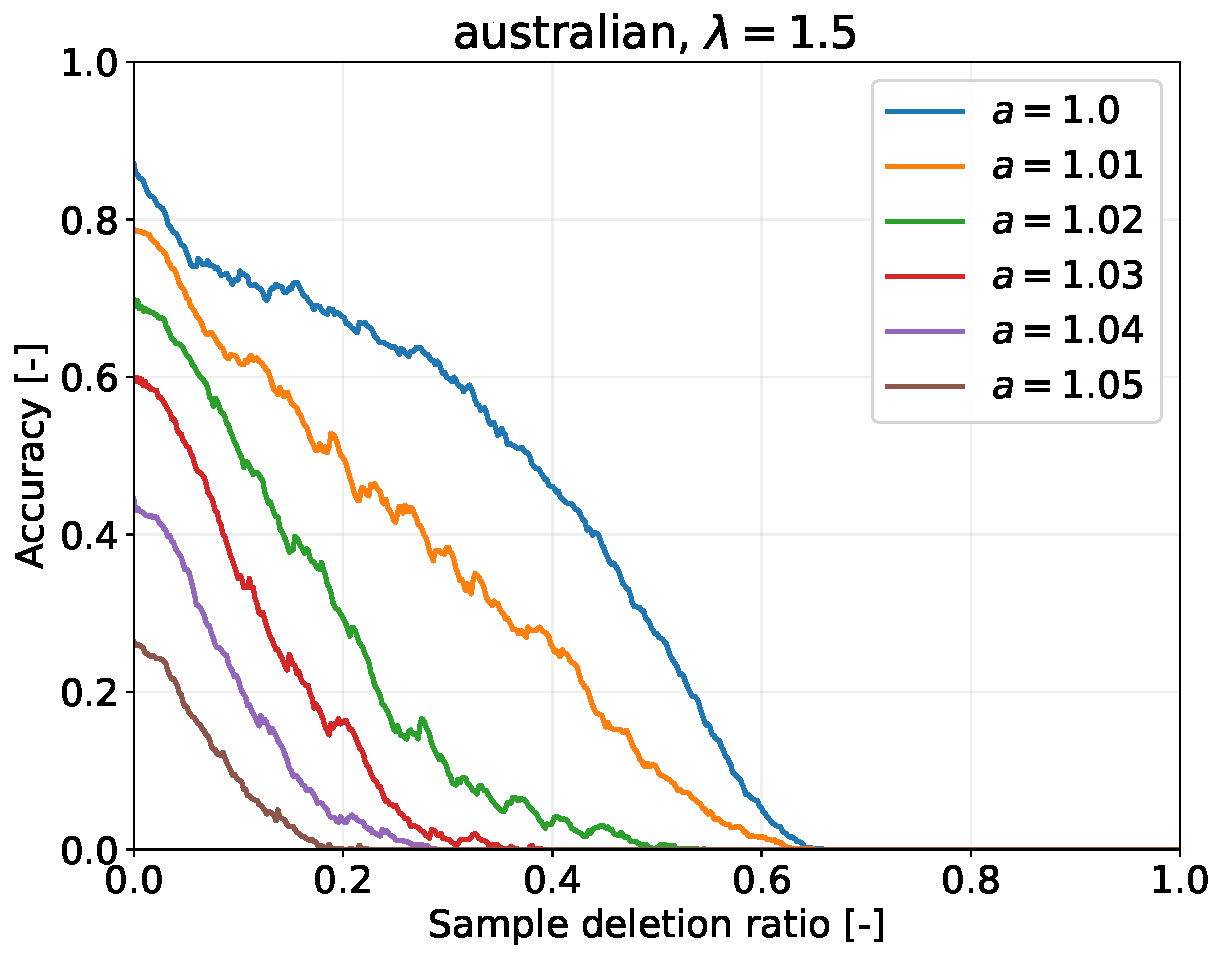
\includegraphics[width=0.30\textwidth]{fig/table_logistic/australian-logistic/kernel/kernel_ss_screening_rate_lam1.5_x_n_y_etest} &
				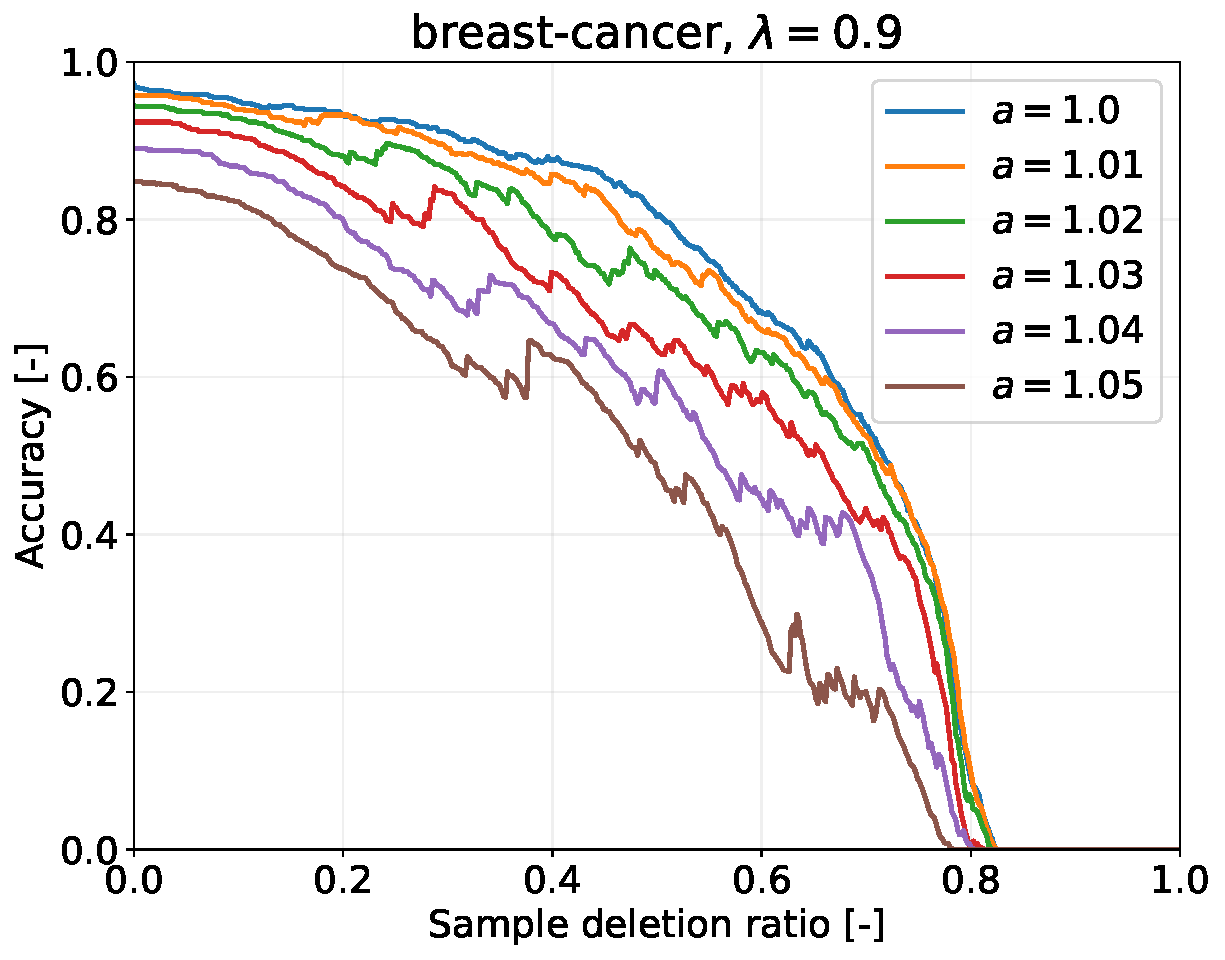
\includegraphics[width=0.30\textwidth]{fig/table_logistic/breast-cancer-logistic/kernel/kernel_ss_screening_rate_lam0.9_x_n_y_etest} &
				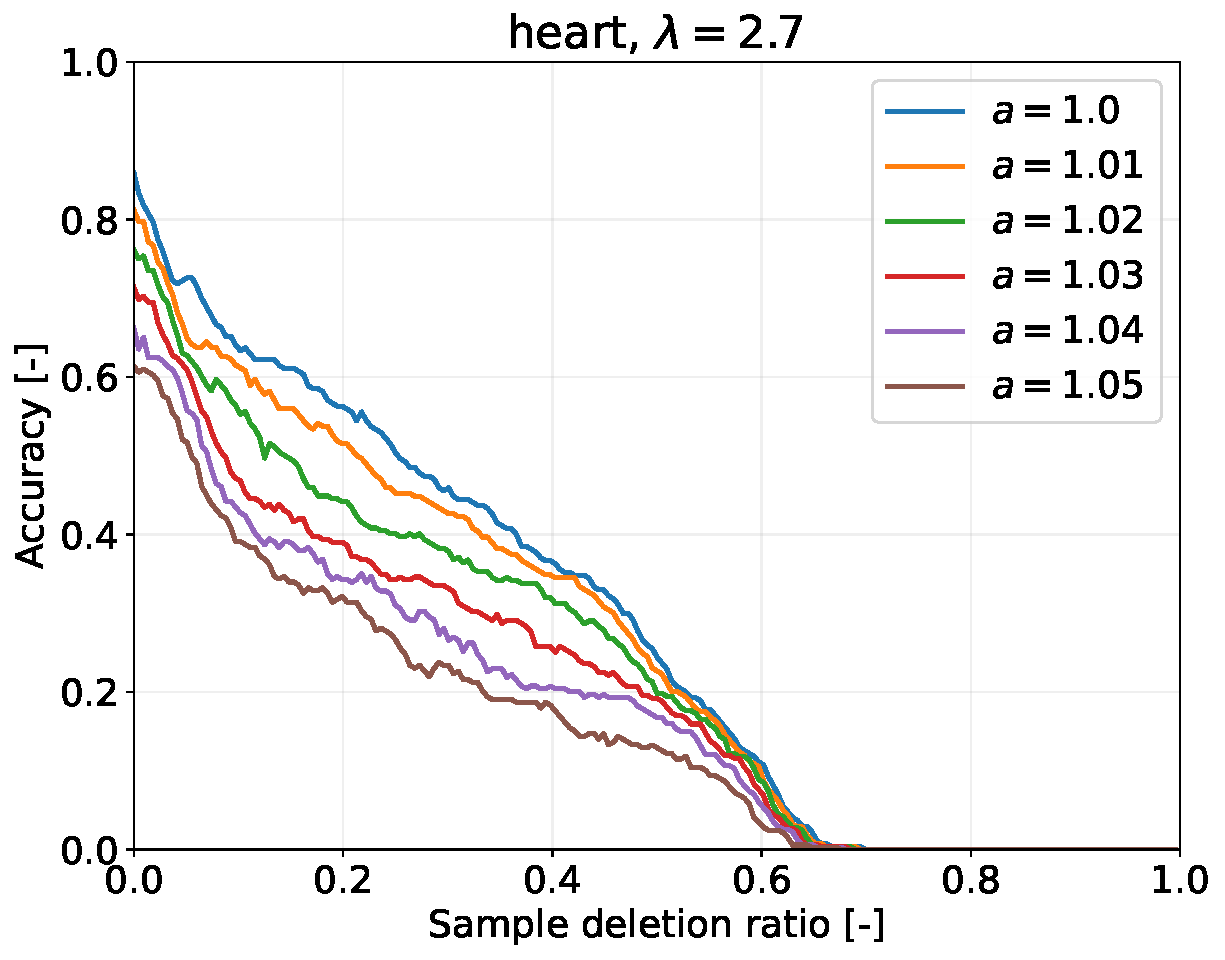
\includegraphics[width=0.30\textwidth]{fig/table_logistic/heart-logistic/kernel/kernel_ss_screening_rate_lam2.7_x_n_y_etest}
			\end{tabular}
		\end{center}
		\caption{We show the lower bound of the worst-case weighted validation accuracy ($1 - {\rm WrVaEr^{\rm UB}}$). This graph indicates that the lower bound of test accuracy is theoretically guaranteed under covariate shift with an unknown test distribution.}
		\label{fig:result-table-guarantee}
	\end{figure}

\subsection{Coreset Selection for Image Data}
	\label{subsec:result-image}
	This section discusses coreset selection for image datasets. As discussed in Section \ref{sec:applicable-class}, although the proposed method is not specifically designed for deep learning, it can be applied to image data by leveraging Neural Tangent Kernels (NTK)\citep{neuraltangents2020} or using the layers preceding the final layer of a deep learning model as a feature extractor.
	%
	In this experiment, considering future extensibility, we apply the proposed method to features extracted from images using a feature extractor.
	%
	The experimental results using NTK are included in the Appendix~\ref{app:result-ntk}.
	%
	In this paper, we evaluate the DRCS method using the CIFAR10 dataset \citep{cifar10}.  
	%  
	CIFAR10 consists of 50,000 training instances and 10,000 test instances, divided into 10 categories.  
	%  
	Since the proposed method is designed for binary classification, we extract a subset of the CIFAR10 dataset.  
	%  
	Specifically, we create a binary classification dataset consisting of 40,000 training instances categorized as vehicles (airplane, automobile, ship, truck) and animals (cat, deer, dog, horse).  
	%  
	The test dataset is similarly divided into two classes, resulting in a total of 8,000 test instances.  
	%  
	The generalization performance of the datasets selected by the coreset selection methods is evaluated using the widely used deep neural network ResNet50 \citep{he2016deep}.  
	%  
	In this experiment, all hyperparameters and experimental settings are kept consistent before and after instance selection and model retraining.  
	%  
	Specifically, for all experiments, we use a batch size of 128, a learning rate of 0.01, weight decay of 0.001, and train the model using the Adam optimizer for 100 epochs.  
	%  
	In the proposed method, the selected instances are transformed using a fixed feature extractor, and classification is performed using the DRCS algorithm.  
	%  
	The feature extractor is trained under the same settings as described in the earlier experimental setup.
	%
	In this experiment for image data, we adopt Algorithm~\ref{alg:2} for calculation of the bound in \eqref{eq:main-bound}.
	
	{\bf Baselines.} The baseline methods for comparing coreset selection are as follows:
	uncertainty-based method:(a)Least Confidence \citep{coleman2019selection}, error/loss-based methods: (b)GraNd \citep{paul2021deep}, (c)DeepFool \citep{ducoffe2018adversarial}, Gradient matching-based method: (d)GradMatch \citep{killamsetty2021grad}, Bilevel optimization-based method: (e)Glister \citep{killamsetty2021glister}, Submodularity-based method: (f)Log-Determinant \citep{iyer2021submodular}.
	For image datasets, comparative experiments were conducted, including methods designed for deep learning.
	%
	In these experiments, the baseline methods were implemented using \citet{guo2022deepcore}.


	The results are shown in Figure~\ref{fig:result-image}.
	%
	The method for visualization and calculation is the same as that used in Section~\ref{subsec:result-table}.
	%
	In this figure, the proposed method demonstrates the higher weighted validation accuracy compared to other methods.


\begin{table}[tb]
	\begin{tabular}{cc}
	\begin{minipage}[t]{0.48\hsize}
	\begin{table}[H]
	\caption{Tabular datasets for numerical experiments. All are binary classification datasets from LIBSVM dataset \citep{libsvmDataset}.}
	\label{tab:dataset-SS}
	\begin{center}
	{\small
	\begin{tabular}{l|rrr}
	\hline
	\multicolumn{1}{c|}{Name} & \multicolumn{1}{c}{$n$} & \multicolumn{1}{c}{$n^+$} & \multicolumn{1}{c}{$d$} \\
	\hline
	splice            &  1000 &  517 & 61 \\
	australian        &  690 &  307 & 15 \\
	breast-cancer     &  683 &  239 & 11 \\
	heart             &  270 &  120 & 14 \\
	ionosphere        &  351 &  225 & 35 \\
	\hline
	\end{tabular}
	}
	\end{center}
	\end{table}
	\end{minipage}
	&
	\begin{minipage}[t]{0.48\hsize}
	\begin{figure}[H]
	\begin{center}
	\begin{tabular}{cc}
	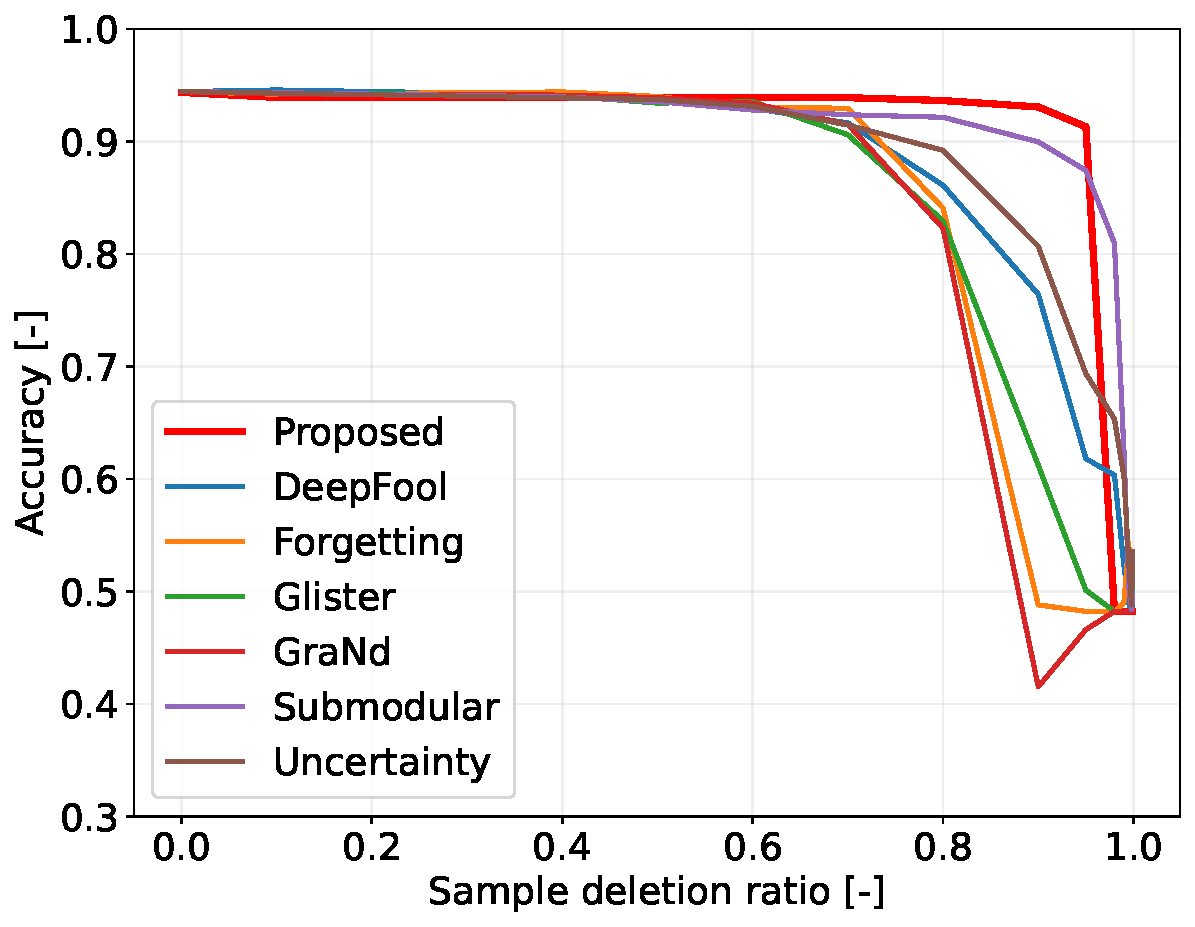
\includegraphics[width=0.8\textwidth]{fig/image/cifar10_1.05.pdf}
	\end{tabular}
	\end{center}
	\caption{We compare our proposed method with several instance selection baselines with respect to the weighted validation accuracy ($1-{\rm VaEr}$). Our method exhibits superior performance generally.}
	\label{fig:result-image}
	\end{figure}
	\end{minipage}
	\end{tabular}
	\end{table}





\subsection{Discussion on Regularization Parameters}
	\label{subsec:discussion-lambda}
	In the previous section, we presented results using a specific preset value for $\lambda$ based on a predefined criterion.
	%
	Ideally, $\lambda$ should be selected to optimize model performance.
	%
	Here, we discuss the relationship between the choice of $\lambda$, the level of theoretical guarantees, and the resulting model performance.
	%
	Here, we present the results for table data.
	\begin{figure}[tb]
		\begin{center}
			\begin{tabular}{cccc}
				\includegraphics[width=0.22\textwidth]{fig/table_logistic/australian-logistic/kernel/lam_0.552/a1.05000.pdf} &
				\includegraphics[width=0.22\textwidth]{fig/table_logistic/australian-logistic/kernel/lam_1.5/a1.05000.pdf} &
				\includegraphics[width=0.22\textwidth]{fig/table_logistic/australian-logistic/kernel/lam_17.45/a1.05000.pdf} &
				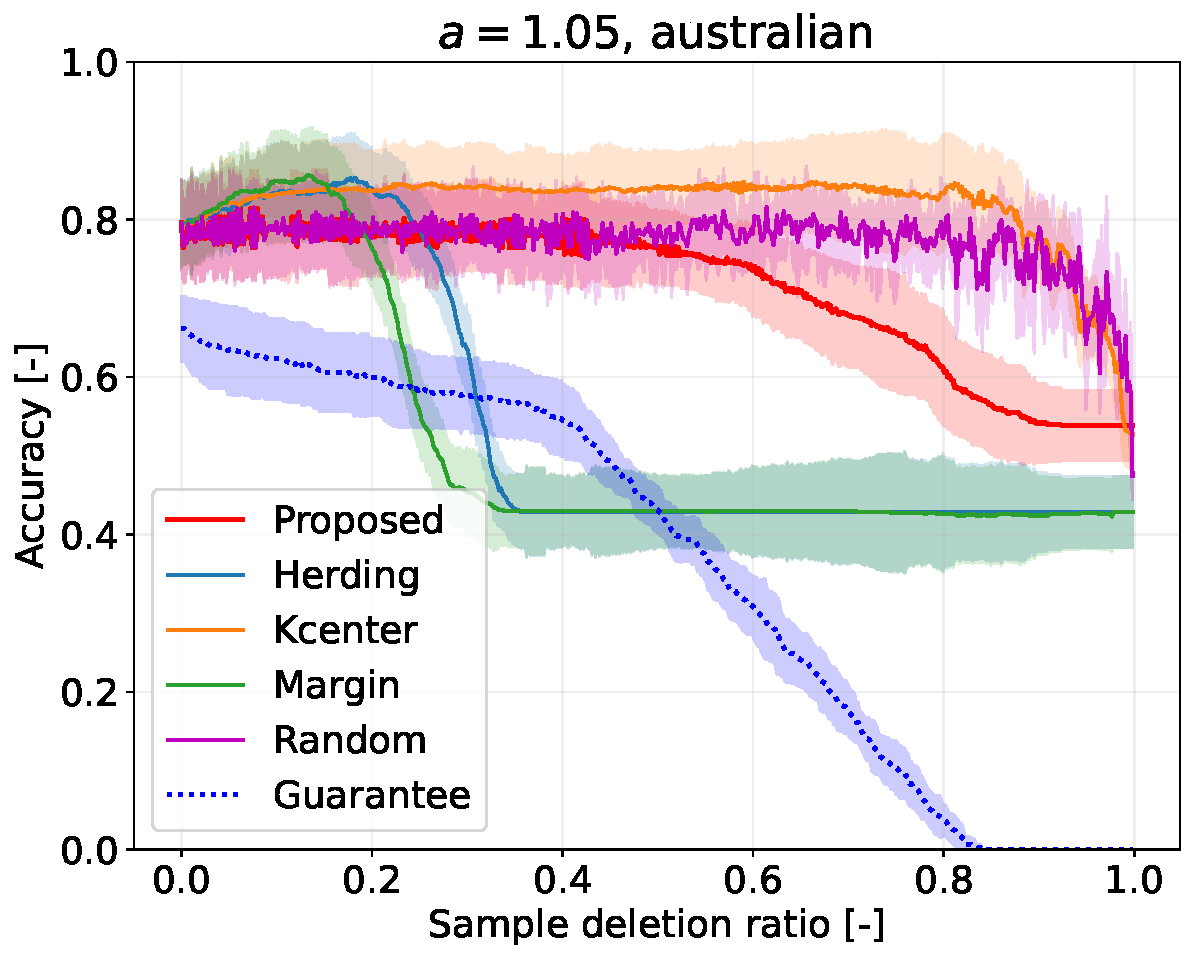
\includegraphics[width=0.22\textwidth]{fig/table_logistic/australian-logistic/kernel/lam_552/a1.05000.pdf} \\
				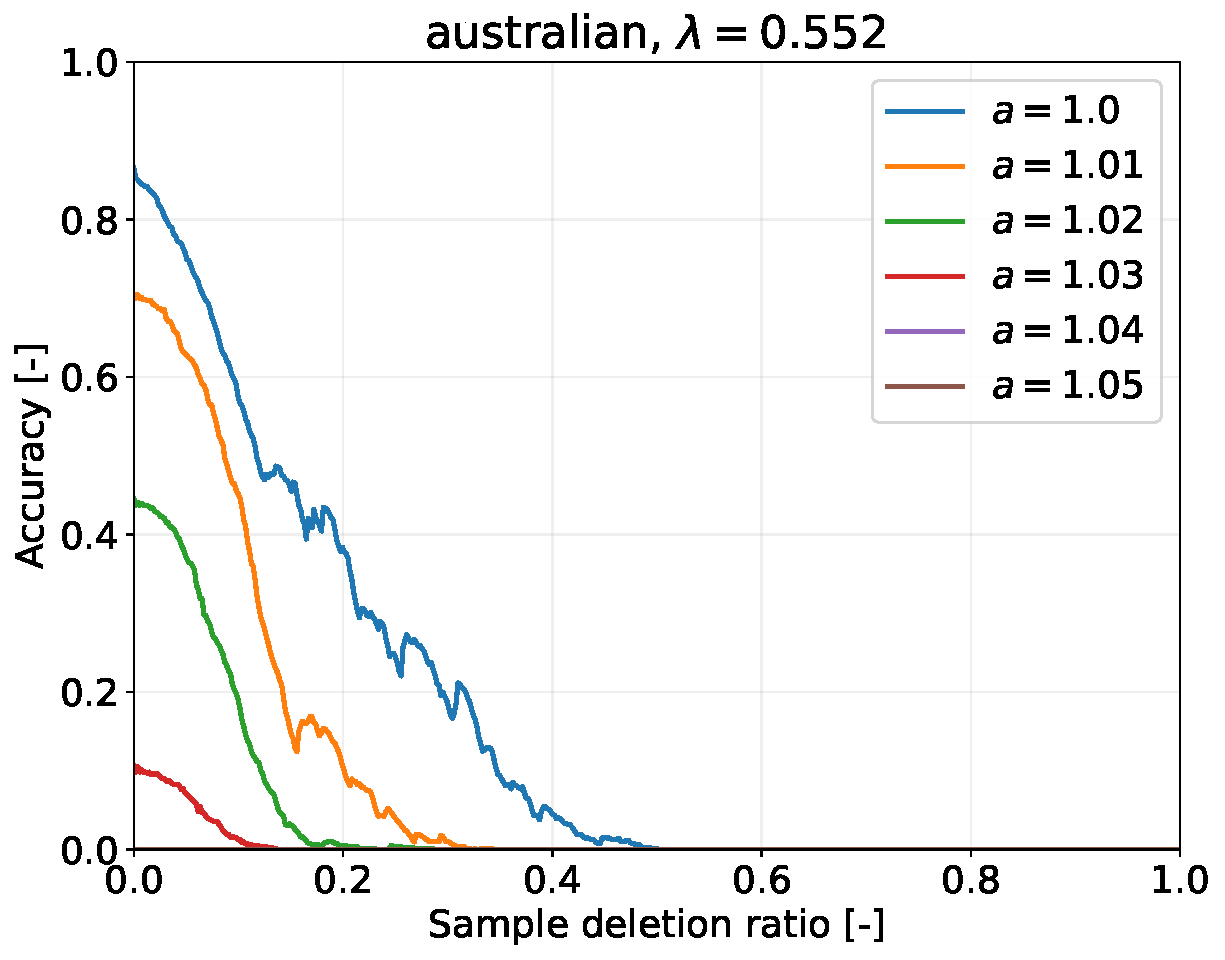
\includegraphics[width=0.22\textwidth]{fig/table_logistic/australian-logistic/kernel/kernel_ss_screening_rate_lam0.552_x_n_y_etest.pdf} &
				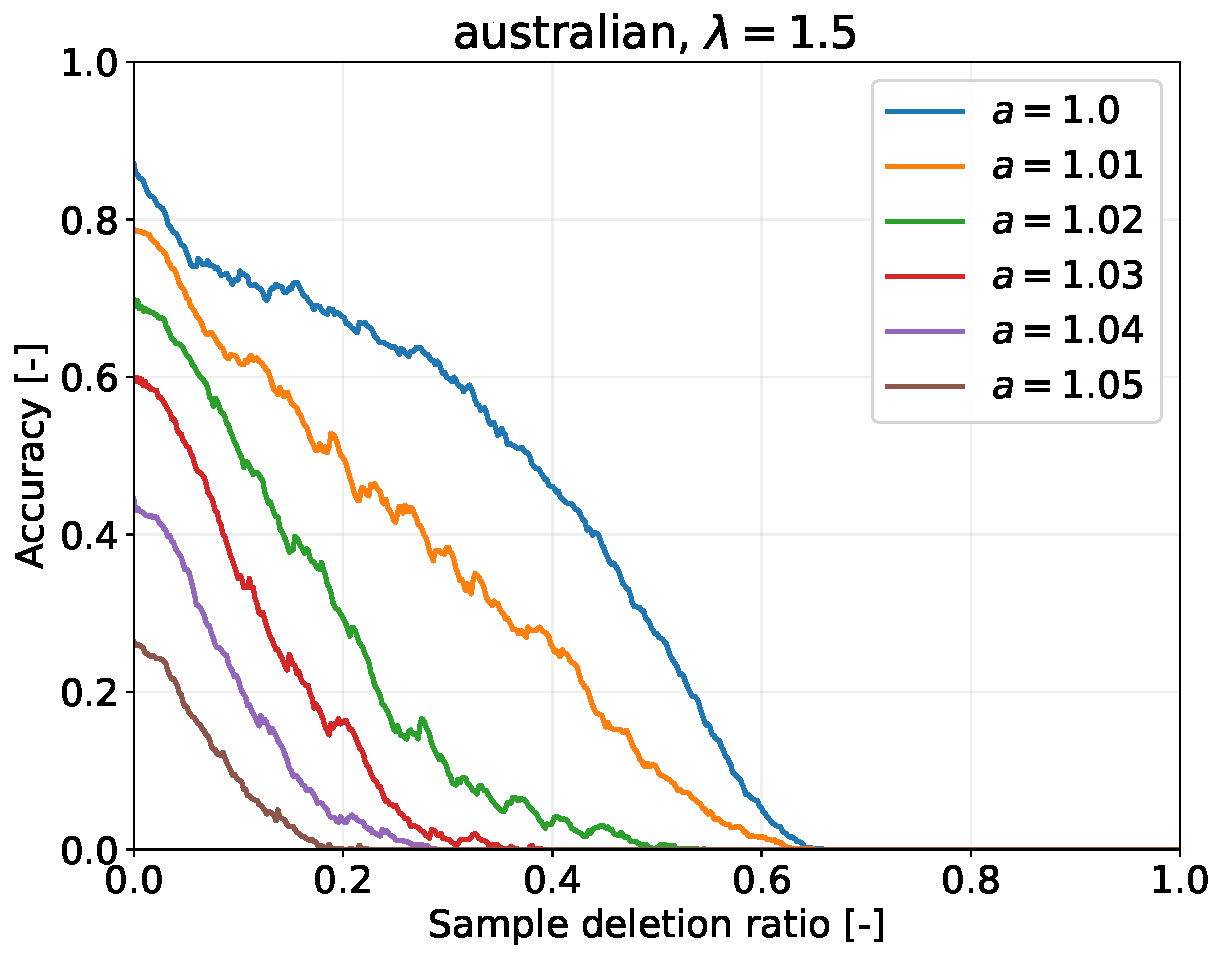
\includegraphics[width=0.22\textwidth]{fig/table_logistic/australian-logistic/kernel/kernel_ss_screening_rate_lam1.5_x_n_y_etest.pdf} &
				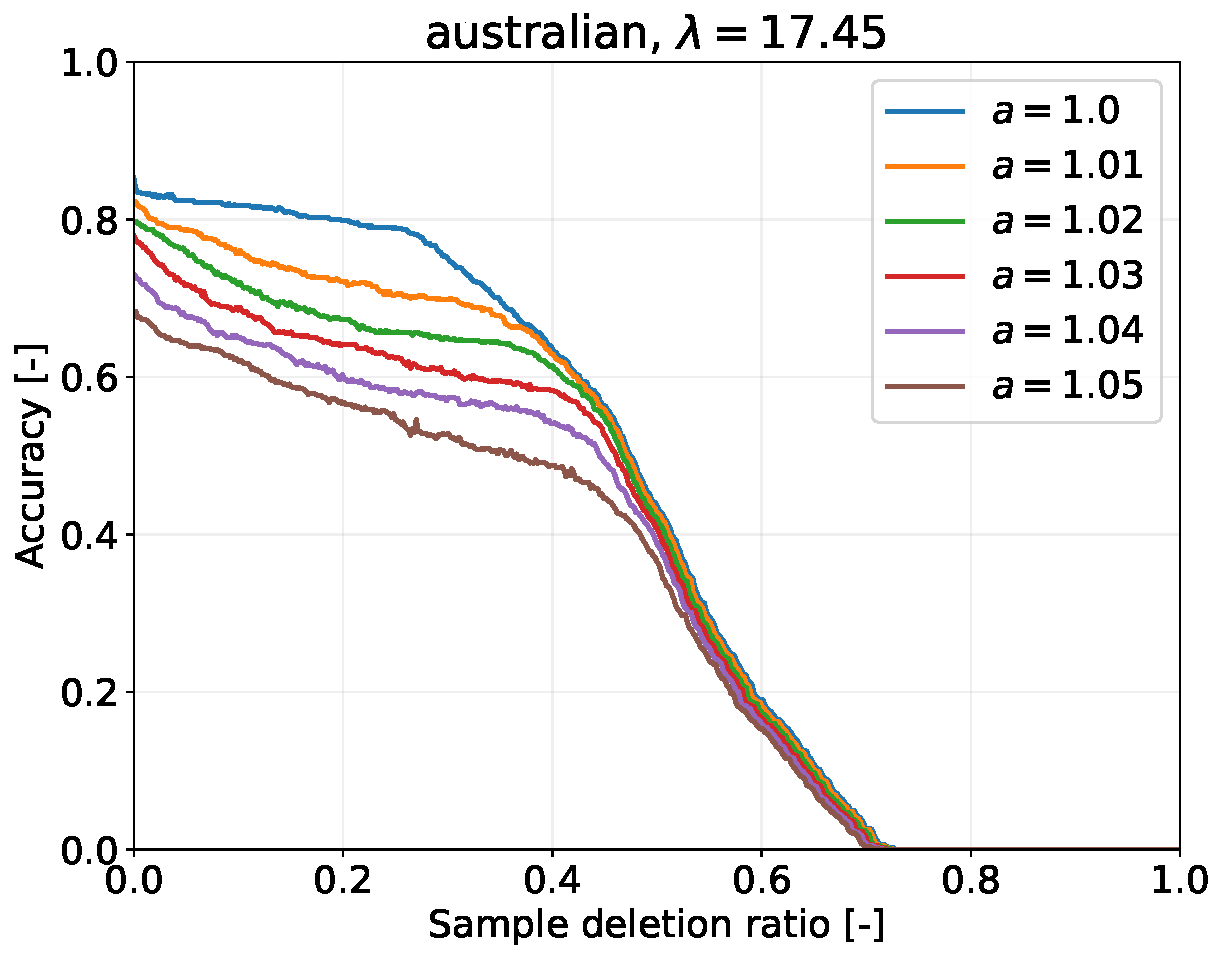
\includegraphics[width=0.22\textwidth]{fig/table_logistic/australian-logistic/kernel/kernel_ss_screening_rate_lam17.45_x_n_y_etest.pdf} &
				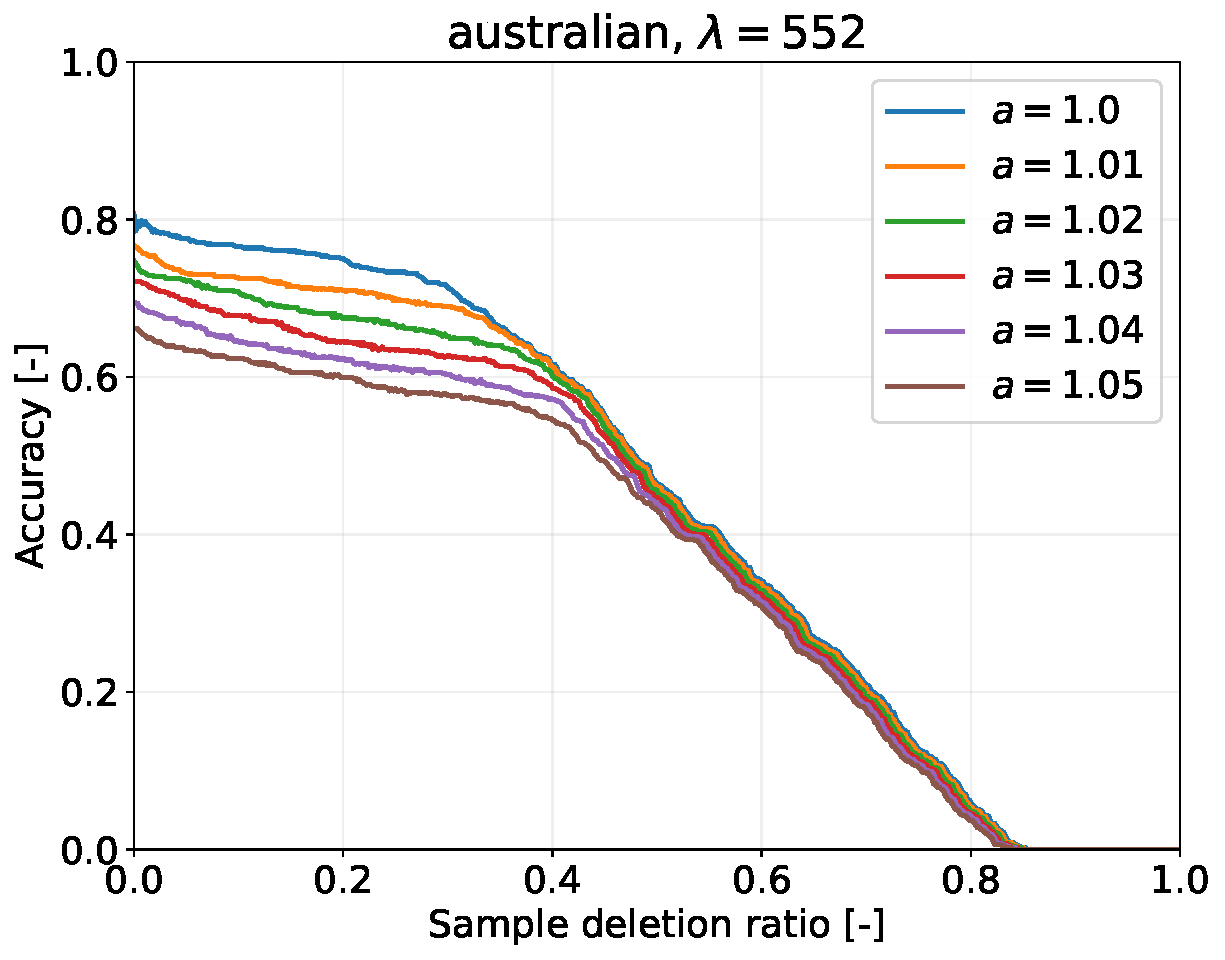
\includegraphics[width=0.22\textwidth]{fig/table_logistic/australian-logistic/kernel/kernel_ss_screening_rate_lam552_x_n_y_etest.pdf}
			\end{tabular}
		\end{center}
		\caption{The results represent the model performance across varying values of lambda. The top row corresponds to the
		weighted validation accuracy ($1-{\rm VaEr}$), and the bottom row to the lower bound of the worst-case weighted validation accuracy ($1-{\rm WrVaEr^{\rm UB}}$). The first column shows results for \(\lambda = n \cdot 10^{-3}\), the second column for \(\lambda = \lambda_{\rm best}\) by cross-validation, the third column for \(\lambda = n \cdot 10^{-1.5}\), and the fourth column for \(\lambda = n\).}
		\label{fig:guarantee}
	\end{figure}

	Figure~\ref{fig:guarantee} illustrates the number of removed instances that can be theoretically guaranteed for specific accuracy levels across different values of $\lambda$.  
	%  
	First, let us compare the columns in the top row of Figure~\ref{fig:guarantee}.  
	%
	In the first and fourth columns, it can be observed that the performance of the proposed method deteriorates in the later stages.
	%
	When strong regularization is applied, the model's performance remains poor even with the entire training set, which diminishes the effectiveness of the proposed method.
	%
	On the other hand, when the regularization is small, the bound of the model parameters becomes broader, making instance selection less effective.
	%

	%
	Second, let us compare the columns in the bottom row of Figure~\ref{fig:guarantee}.
	%  
	In the first column, the model provides strong performance guarantees without any sample deletion or weight change (\(a = 1.0\)).
	%
	However, even slight deletions or small weight changes cause the theoretical guarantees to break down.
	%
	In contrast, in the third and fourth columns, where \(\lambda = n \cdot 10^{-1.5}, n\), the method still provides broader guarantees even with sample deletions or weight changes.
	%
	As the sample deletion ratio increases, the method can provide wider guarantees, although this comes at the cost of reduced guaranteed performance.
	%  
	These observations reveal a trade-off between weight changes, sample deletion ratios, and guaranteed model performance.  
	%  
	This trade-off is likely influenced by the choice of the regularization parameter.  
	%  
	As shown in \eqref{eq:zeta}, a smaller $\lambda$ results in a larger parameter bound, while a larger $\lambda$ leads to a tighter parameter bound.  
	%  
	This effect directly impacts the range of accuracy lower bounds that can be guaranteed.